\chapter{U--Mo fuel: a brief introduction}

%\section{Introduction}\label{sec_ch1_intro}
The Reduced Enrichment for Research and Test Reactors (RERTR)~\cite{snelgrove1997development} program was initiated in the USA in the late 1970s to develop new nuclear fission fuels to replace high-enriched uranium (HEU)\@. The RERTR is now managed by the U.S. National Nuclear Security Administration (NNSA) office of Material Management and Minimization (M$^3$). The development of low-enrichment uranium (LEU) fuels for high-performance reactors is an important nonproliferation initiative as it explained in~\cite{m3web} ``\textit{Material Management and Minimization program reduces the risk of highly enriched uranium and plutonium falling into the hands on nonstate actors by minimizing the use of and, when possible, eliminating weapons-usable nuclear material around the world"}. This initiative has completed a total of 69 reactors conversions to the use of LEU fuel. In addition, 26 reactor facilities have been verified to have been shut down~\cite{wilson2017us}. The conversion of six domestic high performance research reactors~\footnote{Advance Test Reactor at INT, Idaho; Advanced Test Reactor Assembly at INL, Idaho; High Flux Isotope Reactor at ORNL, Tennessee; Massachusetts Institute of Technology Reactor, Massachusetts; National Bureau of Standards Reactor in Gaithersburg, Maryland; University of Missouri Research Reactor in Columbia, Missouri.} that still use Highly Enriched Uranium fuel is yet to be achieved. Due to their unique operating conditions, converting these six reactors is not easy and created a plethora of nuclear engineering challenges. These conversion process may take longer time periods, but developing a new LEU fuel is essential to ensure better performance. 



Research reactors operate at relatively low peak fuel temperatures, but are required to meet fuel performance requirements at high burnup. A typical peak fuel centerline temperature is around 250\textdegree C. For a research reactor fission densities are usually in the range of $3\times10^{21}$ to $6\times10^{21}$ f/cm$^3$. In some cases, peak fuel fission density exceeds $7\times10^{21}$ f/cm$^3$, requiring a higher number of initial $^{235}$U atoms. There are a fewer number of uranium alloys that have the combination of high uranium density and stable fuel behavior to the high burnup to replace the high power density reactors. As it appears, one of the main requirements of LEU fuels is increased uranium density, such as that found in metallic uranium, to offset the decrease in \textsuperscript{235}U enrichment. Metallic uranium is thought to have sufficient density, but the orthorhombic crystal structure of \textalpha-U
and the anisotropic fuel swelling that results make it unattractive as a fuel.
Uranium alloys that retain the high-temperature \textgamma-phase, which is body-centered cubic, are more suitable for reactor fuel due to their more isotropic radiation-induced swelling behavior compared with  \textalpha-uranium~\cite{kittel1993history}.

Various uranium alloys have been tested as alternative metallic fuels under reactor operating conditions, including U$_6$Fe and U$_6$Mn~\cite{meyer2000irradiation,hofman1987irradiation}.
%The U-Mo alloy has been identified as a high-performance fuel due to its high uranium density and low neutron capture cross-section~\cite{ewh2010microstructural,smirnova2013ternary,rest2009analysis,landa2013density}.
Elements such as molybdenum (Mo), niobium (Nb), titanium (Ti), and zirconium (Zr) have also been tried as alloying elements because of their solubility in \textgamma-uranium~\cite{donze1959stabilisation,giraud1973formation,lopes2013mechanical}. Molybdenum stabilizes uranium's \textgamma-phase at concentrations near the eutectoid point, lowering the phase transition temperature from 776~\textdegree C for pure uranium (corresponding to the \textbeta--\textgamma\ allotropic point) to the eutectoid point of 555~\textdegree C for 11.1~percent molybdenum in \textgamma-uranium~\cite{ASM-Alloy-Mo,Berche2011}. To take advantage of this, uranium alloyed with 10 wt$\%$ molybdenum (U-10Mo) is currently being developed as a potential high-density LEU fuel for high-performance research reactors. 

Before the current interest in U--Mo metallic fuel, some of the earlier nuclear reactors used metallic fuel because of the combination of high uranium density and metallic properties. The Godiva IV pulsed reactors at Los Alamos (initially known as \textit{Lady Godiva}) used U--Mo alloys, which dates back to 1960. The Fast Burst Reactor (FBR) at White Sands, the Army Pulsed Radiation Facility (Aberdeen, MD), and the Sandia Pulsed Reactor II used U--Mo alloys. All of these reactors utilized the \textgamma~phase of uranium, but because of the short irradiation time the impacts of fuel burnup were minimal~\cite{horak1973operating}. The Dounreay Fast Reactor used a number of metal-fuel-based designs, which inclueds U-9.1 wt\% Mo and U-7 wt\% Mo clad in niobium. The highly alloyed fuel cracked more, even though the 9.1-wt\%-Mo fuel swelled slightly less than 7 wt\%-Mo alloy~\cite{cottrell1964development}. In U.S. the Enrico Fermi Fast Breeder Reactor (EFFBR) was the first commercial fast reactor that used U--10Mo fuel. The primary concern was to ensure that the fuel would maintain \textgamma-phase stability during the operating condition. A series of experiments have been performed and mapped the fission rate and temperature dependence of \textgamma-phase stability~\cite{no20031374}. Two types of U--Mo alloy fuel have been designed and tested. One is monolithic fuel form, in which a thin layer of U--Mo foil is bonded to aluminum clad. The other is a dispersion fuel form, where U--Mo/Al, composed of U--Mo fuel particles that are dispersed in an inert Al matrix.

\begin{figure}
\centering
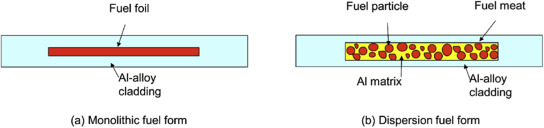
\includegraphics[scale=1.0]{dispersion_monolithic.jpg}
\caption[Schematic of monolithic and dispersion fuel]{Schematic diagram for monolithic and dispersion fuel from Jeong \etal~\cite{jeong2015mechanical}}
\end{figure}
 

For five decades, the dispersion fuel has powered many test and research reactors worldwide. The manufacturing process and operating conditions are well known for these types of fuels. One of the first experimental work performed for U--Mo fuel was performed on U--Mo dispersion fuel. The high-burnup testing of the dispersion fuel showed a pattern of breakaway swelling (also called `blistering' or `pillowing') behavior at intermediate burnup. The post-irradiation examination (pie) of the U--Mo dispersion fuel revealed that this phenomenon is due to fission gas released from the interaction layer. Reaction between the U--Mo and aluminum occurs during irradiation and forms a ternary alumnide [(U--Mo)Al$_x$] phase which releases the fission gas at the boundary between the interaction phase and the aluminum matrix~\cite{leenaers2004post,jue2014microstructural,van2008transmission, olander2009growth}. These gas bubbles have tendency to aggregate into the gas pockets, which weakens the fuel meat by exerting internal gas pressure. The result is a mechanical failure and large increase of the fuel volume. To eliminate the fuel matrix interaction the `monolithic' U--Mo fuel was suggested. In monolithic fuels, a zirconium foil is used as a diffusion barrier between the fuel and the cladding (aluminum) to prevent diffusion of molybdenum into the cladding~\cite{jue2014microstructural}.


In the current work we have investigated how fission gas (xenon and krypton) impacts the U--Mo fuel. In the second chapter we have studied the reduction of thermal conductivity due to the presence of xenon gas. We have implemented finite element method to study the different microstructural configuration of fission gas in U--Mo fuel. In the third chapter we have introduced a new \textit{pseudopotential} for metallic uranium to study the properties using first-principles (Density Functional Theory (DFT)) method. In the fourth chapter we will discuss about the atomistic diffusion mechanism of xenon in U--Mo fuel, which includes the study of xenon gas in the U--Mo fuel using DFT methods. 
















\bibliographystyle{unsrt}
\bibliography{abbreviated,comp}
